\documentclass[journal,twocolumn]{IEEEtran}

\usepackage[T1]{fontenc}
\usepackage[utf8]{inputenc}
\usepackage{amsmath,amssymb,amsfonts}
\usepackage{graphicx}
\usepackage{booktabs}
\usepackage{multirow}
\usepackage{xcolor}
\usepackage{url}
\usepackage{hyperref}
\usepackage{caption}
\usepackage{subcaption}
\usepackage{float}
\usepackage{algorithm}
\usepackage{algorithmic}
\usepackage{array}
\usepackage{tabularx}
\usepackage{balance}

\hypersetup{
  colorlinks=true,
  linkcolor=black,
  citecolor=black,
  urlcolor=black
}

\newcolumntype{C}[1]{>{\centering\arraybackslash}p{#1}}

\begin{document}

\title{Webshell Detection Using Classical Machine Learning:\\
Feature Engineering, Dimensionality Reduction, and Cost-Sensitive Boosting}

\author{
  \IEEEauthorblockN{Sara Allab}
  \IEEEauthorblockA{
    National Higher School of Mathematics (NHSM)\\
    Algiers, Algeria\\
    \textit{s.allab@nhsm.edu.dz}
  }
}

\maketitle

\begin{abstract}
Webshells are malicious scripts injected into compromised web servers to enable persistent remote access and privilege escalation. Their detection is a critical challenge in web security because attackers continuously evolve evasion techniques such as code encryption, obfuscation, and functional splitting. This paper presents a systematic machine learning study for PHP webshell detection across three experimental phases. In Phase I, five classical classifiers---Decision Tree (DT), K-Nearest Neighbors (KNN), Support Vector Machine (SVM), Naive Bayes (NB), and Logistic Regression (LR)---are trained on two pre-extracted feature datasets (D1 and D2) with and without Principal Component Analysis (PCA). In Phase II, a custom feature extraction pipeline is implemented on 6,134 raw PHP files from the WhiteBlackPHP dataset, combining statistical, syntactical, and lexical features; seven classifiers are evaluated including Random Forest (RF) and a cost-sensitive AdaCost ensemble. Random Forest achieves the highest performance across all experiments, reaching an F1-score of 0.9656 and an AUC of 0.9951 on the WhiteBlackPHP dataset without feature selection. PCA reduces accuracy for most models, while lexical and statistical features prove most discriminative for webshell identification.
\end{abstract}

\begin{IEEEkeywords}
webshell detection, PHP malware, machine learning, feature engineering, AdaCost, cost-sensitive learning, Random Forest, intrusion detection
\end{IEEEkeywords}

% ============================================================
\section{Introduction}
% ============================================================

A webshell is a script---commonly written in PHP, JSP, ASP, or ASPX---that an attacker uploads to a compromised web server. Once deployed, it provides a persistent, browser-accessible backdoor through which an adversary can execute arbitrary operating system commands, read and exfiltrate sensitive data, pivot deeper into internal networks, and escalate privileges. Unlike traditional malware, webshells are indistinguishable at a glance from legitimate server-side scripts, making signature-based antivirus tools largely ineffective.

The challenge is compounded by four well-documented evasion techniques. \textit{Letter slicing} fragments dangerous function names (e.g., \texttt{ev} $+$ \texttt{al}) into sub-strings that are concatenated at runtime. \textit{Code encryption} wraps payloads in \texttt{base64\_decode} or custom XOR routines. \textit{Code confusing} floods a file with dummy variables and dead branches. \textit{Code splitting} distributes a webshell across multiple files linked by \texttt{include()} or \texttt{require()}, defeating single-file analysis.

Machine learning approaches address these limitations by learning discriminative statistical and structural patterns directly from file content rather than relying on brittle, manually curated signatures. The core hypothesis, validated extensively in the literature \cite{wang2012detecting,wang2015detecting}, is that malicious PHP code exhibits measurable differences from benign code along several dimensions: higher Shannon entropy (due to obfuscation), longer base64-encoded tokens, higher frequencies of dangerous function calls, and unusual control-flow structures.

This paper makes the following contributions:
\begin{itemize}
  \item A rigorous three-phase experimental evaluation of five classical and two ensemble classifiers on three independent PHP datasets.
  \item A modular feature extraction pipeline covering statistical (entropy, index of coincidence, compression ratio), syntactical (string counts, line metrics), and lexical (dangerous functions, commands, variables, keywords) features, producing 87 features per file.
  \item A from-scratch implementation of the AdaCost cost-sensitive boosting algorithm \cite{fan1999adacost}, designed to penalise missed webshell detections more heavily than false positives.
  \item Systematic comparison of the impact of PCA and SelectKBest feature selection on detection performance.
\end{itemize}

% ============================================================
\section{Related Work}
% ============================================================

Early webshell detectors relied purely on keyword blacklists and regular-expression matching. Whilst trivially bypassed by letter slicing, these methods established the taxonomy of dangerous PHP constructs that later feature-engineering work formalised.

Wang et al.\ \cite{wang2012detecting} were among the first to cast webshell detection as a supervised classification problem, extracting token-frequency features from PHP abstract syntax trees and training a Na\"{i}ve Bayes model. Their work demonstrated recall above 90\% on a small curated corpus but noted significant degradation on obfuscated samples.

The neopi tool \cite{neopi2010} introduced information-theoretic features---Shannon entropy, index of coincidence, and compression ratio---specifically tailored to detect encrypted or encoded payloads. These features form the statistical backbone of our feature set.

More recent studies have explored deep learning alternatives. Tian et al.\ \cite{tian2020}, for instance, applied bidirectional LSTM networks to opcode sequences, achieving competitive results but at significantly higher computational cost. Our work demonstrates that classical methods, when combined with rich hand-crafted features and well-tuned hyperparameters, remain highly competitive and far more interpretable.

The WhiteBlackPHP dataset used in Phase II was introduced by \cite{dataset2022} and represents one of the largest publicly available collections of labelled PHP files, with near-duplicate removal achieved through both MD5 hashing and VLD opcode comparison.

% ============================================================
\section{Datasets}
% ============================================================

Three datasets are used across the two experimental phases, as summarised in Table~\ref{tab:datasets}.

\begin{table}[H]
\centering
\caption{Dataset Summary}
\label{tab:datasets}
\begin{tabular}{@{}lccccc@{}}
\toprule
Dataset & Dedup & Normal & Webshell & Total & Format \\
\midrule
D1 & MD5 & 1{,}411 & 1{,}962 & 3{,}373 & Pre-extracted \\
D2 & MD5+VLD & 1{,}119 & 1{,}119 & 2{,}238 & Pre-extracted \\
WhiteBlackPHP & MD5+VLD & 3{,}067 & 3{,}067 & 6{,}134 & Raw PHP \\
\bottomrule
\end{tabular}
\end{table}

\textbf{D1} was constructed by crawling public GitHub repositories and webshell collections, deduplicating files by MD5 hash. The resulting set is imbalanced, with webshells outnumbering normal files by a ratio of roughly 1.4:1.

\textbf{D2} applies an additional deduplication step using VLD (Vulcan Logic Disassembler) opcode comparison to remove \textit{near-duplicates}---files that differ only in formatting or whitespace but encode identical logic. This yields a perfectly balanced binary classification problem.

\textbf{WhiteBlackPHP} is the largest and most challenging dataset. It exposes raw PHP source code rather than pre-extracted features, requiring a full feature extraction pipeline (Section~\ref{sec:features}). Its balance and size make it the primary benchmark for Phase II.

Fig.~\ref{fig:class_dist} shows the class distributions for D1 and WhiteBlackPHP. The imbalance in D1 is visible and motivates the use of stratified cross-validation throughout.

\begin{figure}[H]
  \centering
  \begin{subfigure}[b]{0.48\linewidth}
    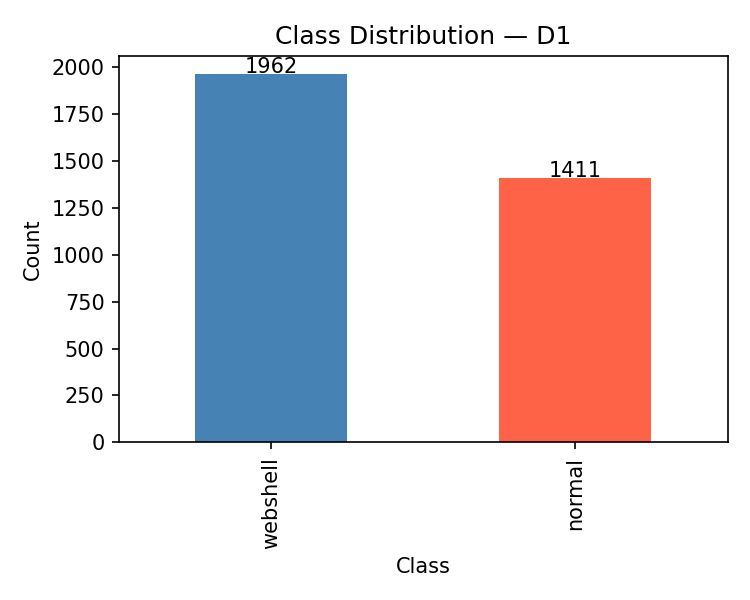
\includegraphics[width=\linewidth]{results/figures/D1_class_dist.png}
    \caption{D1}
  \end{subfigure}
  \hfill
  \begin{subfigure}[b]{0.48\linewidth}
    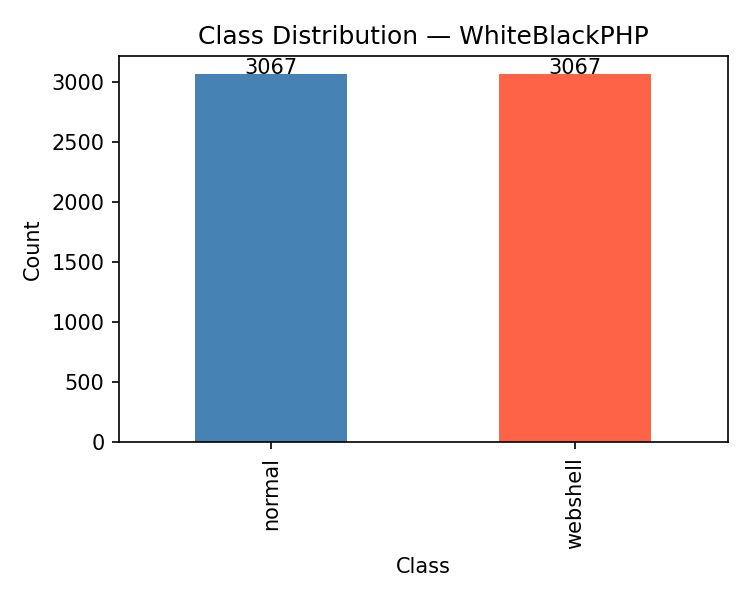
\includegraphics[width=\linewidth]{results/figures/part2_class_dist.png}
    \caption{WhiteBlackPHP}
  \end{subfigure}
  \caption{Class distributions. D1 is imbalanced (1,411 normal vs.\ 1,962 webshells). WhiteBlackPHP is perfectly balanced.}
  \label{fig:class_dist}
\end{figure}

% ============================================================
\section{Methodology}
\label{sec:method}
% ============================================================

\subsection{Feature Engineering}
\label{sec:features}

The feature extraction pipeline operates directly on raw PHP source code and produces 87 numeric features per file, organised into three groups.

\subsubsection{Statistical Features}

Inspired by the neopi framework \cite{neopi2010}, five information-theoretic measures capture the degree of obfuscation or encryption present in a file.

\textbf{Shannon Entropy} measures the randomness of byte distribution:
\begin{equation}
  H(X) = -\sum_{i} p_i \log_2 p_i
  \label{eq:entropy}
\end{equation}
Encrypted or base64-encoded payloads produce values close to 8 bits, whereas natural PHP source code typically falls between 4 and 6 bits.

\textbf{Index of Coincidence (IC)} measures how non-uniform the character frequency distribution is:
\begin{equation}
  IC = \frac{\sum_i f_i(f_i - 1)}{n(n-1)}
  \label{eq:ic}
\end{equation}
where $f_i$ is the frequency of character $i$ and $n$ is the total character count. Encrypted text yields a low IC; natural language or structured code yields a higher IC.

\textbf{Longest Word} reports the maximum token length after splitting on non-alphanumeric characters. Base64-encoded strings produce very long unbroken token sequences.

\textbf{Compression Ratio} is the ratio of zlib-compressed file size to original size. Repetitive, structured code compresses well; random-looking obfuscated code does not.

\textbf{Signature Count} counts how many of the 29 known dangerous functions from the neopi nasty list appear in the file.

\subsubsection{Syntactical Features}

Seven features capture structural properties of the PHP source code independent of specific function names:

\begin{itemize}
  \item \textit{total\_size}: file size in bytes.
  \item \textit{nb\_string}: number of quoted string literals.
  \item \textit{nb\_neq\_string}: number of \textit{unique} string literals.
  \item \textit{nb\_special\_char}: count of non-alphanumeric, non-whitespace characters.
  \item \textit{max\_length\_line}: length of the longest line (obfuscated code tends to pack everything onto a single line).
  \item \textit{nb\_if}: count of \texttt{if(} occurrences.
  \item \textit{nb\_loop}: count of \texttt{for/while/foreach(} occurrences.
\end{itemize}

\subsubsection{Lexical Features}

The lexical group provides binary occurrence counts for 75 patterns known to be associated with webshell activity, drawn from the literature and from the dataset's own annotation:

\begin{itemize}
  \item 47 \textbf{dangerous functions}: \texttt{eval}, \texttt{base64\_decode}, \texttt{base64\_encode}, \texttt{shell\_exec}, \texttt{system}, \texttt{exec}, \texttt{proc\_open}, \texttt{passthru}, \texttt{assert}, \texttt{unserialize}, \texttt{popen}, \texttt{curl\_exec}, etc.
  \item 16 \textbf{dangerous shell commands}: \texttt{wget}, \texttt{gcc}, \texttt{chmod}, \texttt{nc}, \texttt{uname}, \texttt{whoami}, \texttt{perl}, \texttt{python}, etc.
  \item 10 \textbf{dangerous superglobal variables}: \texttt{\$\_GET}, \texttt{\$\_POST}, \texttt{\$\_COOKIE}, \texttt{\$\_REQUEST}, \texttt{\$\_FILES}, \texttt{\$cmd}, etc.
  \item 16 \textbf{known webshell keywords}: \textit{webshell by}, \textit{c99shell}, \textit{r57}, \textit{phpspy}, \textit{n3shell}, etc.
\end{itemize}

\subsection{Preprocessing}

The preprocessing pipeline is applied identically in all experiments:
\begin{enumerate}
  \item \textbf{Imputation}: missing or non-numeric values are replaced by the feature-wise median.
  \item \textbf{Standardisation}: zero-mean, unit-variance scaling via \texttt{StandardScaler}.
  \item \textbf{Stratified split}: 80\% train / 20\% test with class-proportion preservation.
\end{enumerate}

In the PCA experiments (Phase I), Principal Component Analysis is applied after standardisation, retaining enough components to explain 95\% of the variance. In the feature-selection experiments (Phase II), \texttt{SelectKBest} with the $F$-score statistic selects the top 30 features.

\subsection{Classifiers}

\textbf{Decision Tree (DT)} partitions the feature space by recursive binary splits. Grid-searched over \texttt{max\_depth} $\in \{3, 5, 10, \infty\}$, \texttt{min\_samples\_split} $\in \{2, 5, 10\}$, and criterion $\in \{\text{Gini}, \text{Entropy}\}$.

\textbf{K-Nearest Neighbours (KNN)} classifies a sample by majority vote among its $k$ nearest neighbours in feature space. Grid-searched over $k \in \{3, 5, 7, 11, 15\}$, distance metrics $\in \{\text{Euclidean}, \text{Manhattan}\}$, and weight schemes $\in \{\text{uniform}, \text{distance}\}$.

\textbf{Support Vector Machine (SVM)} finds the maximum-margin hyperplane. Grid-searched over $C \in \{0.1, 1, 10, 100\}$, kernels $\in \{\text{RBF}, \text{linear}\}$, and $\gamma \in \{\text{scale}, \text{auto}\}$.

\textbf{Na\"{i}ve Bayes (NB)} assumes conditional feature independence given the class label and models each feature as Gaussian. Grid-searched over the variance smoothing parameter.

\textbf{Logistic Regression (LR)} fits a linear decision boundary in the standardised feature space. Grid-searched over $C \in \{0.01, 0.1, 1, 10, 100\}$ and solvers \texttt{lbfgs}/\texttt{liblinear}.

\textbf{Random Forest (RF)} aggregates predictions from 100--300 decorrelated decision trees via bagging. Grid-searched over \texttt{n\_estimators}, \texttt{max\_depth}, and \texttt{max\_features}.

\textbf{AdaCost} \cite{fan1999adacost} is a cost-sensitive extension of AdaBoost. It modifies the weight update rule to penalise false negatives (missed webshells) more heavily than false positives. At each boosting round $t$, weak learner $h_t$ is fitted to the current weight distribution, and sample weights are updated as:

\begin{equation}
  w_i \leftarrow w_i \cdot \exp\!\bigl(\alpha_t \cdot \mathbb{1}[h_t(x_i) \neq y_i] \cdot \beta(y_i, h_t(x_i))\bigr)
  \label{eq:adacost}
\end{equation}

where $\alpha_t = \frac{1}{2}\ln\!\frac{1-\varepsilon_t}{\varepsilon_t}$ is the round weight, $\varepsilon_t$ is the weighted error rate, and $\beta$ is the cost multiplier: $\beta = c^+$ for false negatives and $\beta = c^-$ for false positives, with $c^+ \geq c^-$. Grid-searched over \texttt{n\_estimators} $\in \{50, 100, 200\}$ and $c^+ \in \{1, 2, 3, 5\}$.

\subsection{Evaluation Protocol}

All hyperparameters are selected via \textbf{5-fold stratified cross-validation GridSearchCV} on the training set, optimising the F1-score. Final metrics---Accuracy, Precision, Recall, F1, and AUC---are computed on the held-out test set:
\begin{align}
  \text{Precision} &= \frac{TP}{TP + FP} \\
  \text{Recall}    &= \frac{TP}{TP + FN} \\
  F_1             &= \frac{2 \cdot \text{Precision} \cdot \text{Recall}}{\text{Precision} + \text{Recall}} \\
  \text{AUC}       &= \int_0^1 \text{TPR}(\text{FPR})\,d\text{FPR}
\end{align}

% ============================================================
\section{Phase I: Pre-Extracted Feature Datasets}
% ============================================================

\subsection{Results on D1}

Table~\ref{tab:d1} reports the five classifier performance scores on the D1 dataset, with and without PCA.

\begin{table}[H]
\centering
\caption{Phase I results on D1 (3,373 samples). Best per column in \textbf{bold}.}
\label{tab:d1}
\renewcommand{\arraystretch}{1.15}
\begin{tabular}{@{}llccccc@{}}
\toprule
 & Model & Acc & Pre & Rec & F1 & AUC \\
\midrule
\multirow{5}{*}{\rotatebox{90}{Raw}}
 & DT   & \textbf{.954} & \textbf{.976} & .944 & \textbf{.960} & .955 \\
 & KNN  & .948 & .974 & .936 & .955 & .975 \\
 & SVM  & .948 & .961 & .949 & .955 & \textbf{.982} \\
 & NB   & .776 & .980 & .629 & .766 & .946 \\
 & LR   & .941 & .961 & .936 & .948 & .980 \\
\midrule
\multirow{5}{*}{\rotatebox{90}{PCA}}
 & DT   & .935 & .958 & .929 & .943 & .933 \\
 & KNN  & .948 & .976 & .934 & .955 & \textbf{.983} \\
 & SVM  & .941 & .958 & .939 & .949 & .974 \\
 & NB   & .662 & .966 & .435 & .600 & .922 \\
 & LR   & .919 & .942 & .916 & .929 & .976 \\
\bottomrule
\end{tabular}
\end{table}

On the raw D1 features, Decision Tree achieves the highest F1-score (0.960) while SVM achieves the highest AUC (0.982), indicating superior probabilistic calibration. All models except Na\"{i}ve Bayes exceed 94\% accuracy. NB achieves near-perfect precision (0.980) but suffers catastrophic recall (0.629), meaning it misses roughly one in three webshells---a critical failure mode in security applications.

After PCA, most models show a modest accuracy decline (1--2 percentage points), consistent with the information loss inherent in dimensionality reduction. Notably, KNN actually improves its AUC from 0.975 to 0.983 under PCA, suggesting that the removal of noisy high-variance dimensions benefits distance-based classifiers.

Fig.~\ref{fig:d1_roc} presents the ROC curves for both D1 configurations.

\begin{figure}[H]
  \centering
  \begin{subfigure}[b]{0.48\linewidth}
    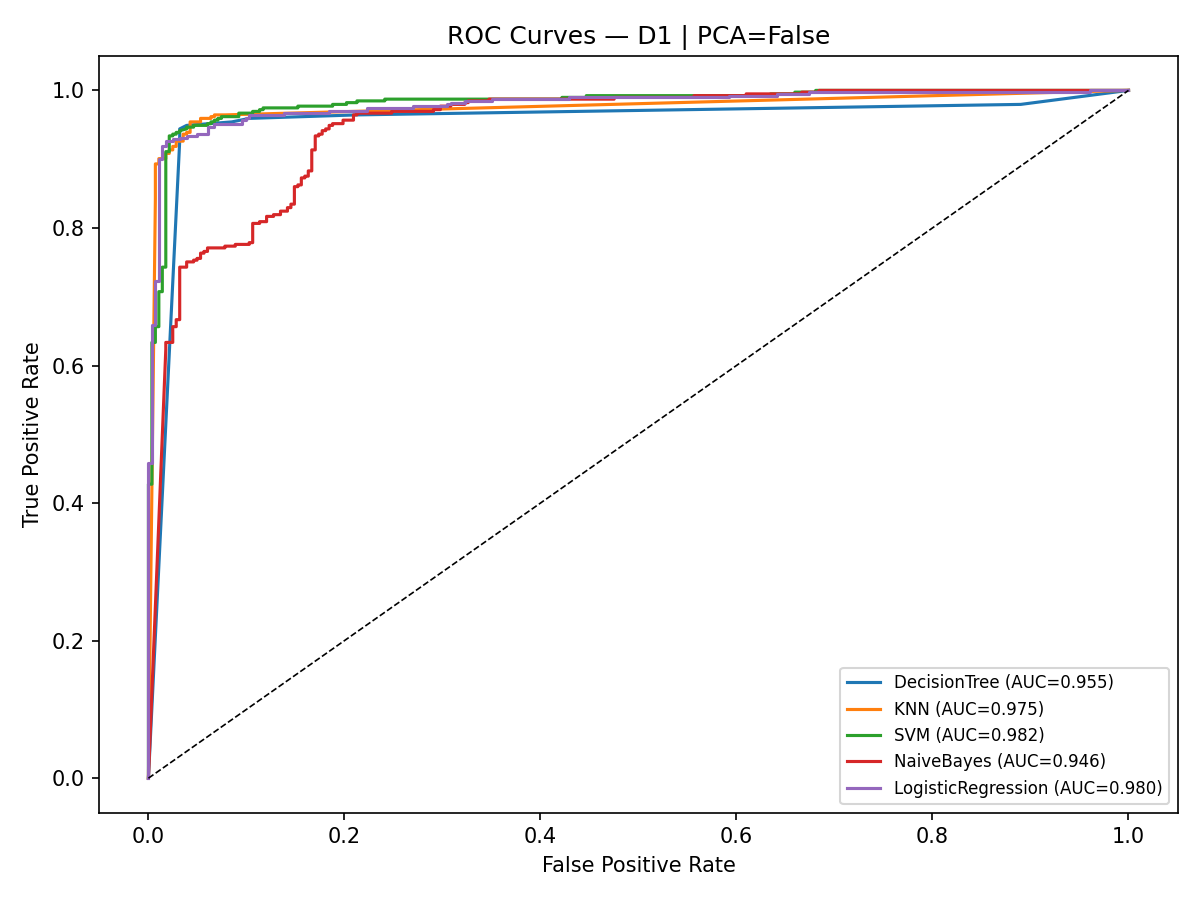
\includegraphics[width=\linewidth]{results/figures/D1_raw_roc.png}
    \caption{D1 — Raw features}
  \end{subfigure}
  \hfill
  \begin{subfigure}[b]{0.48\linewidth}
    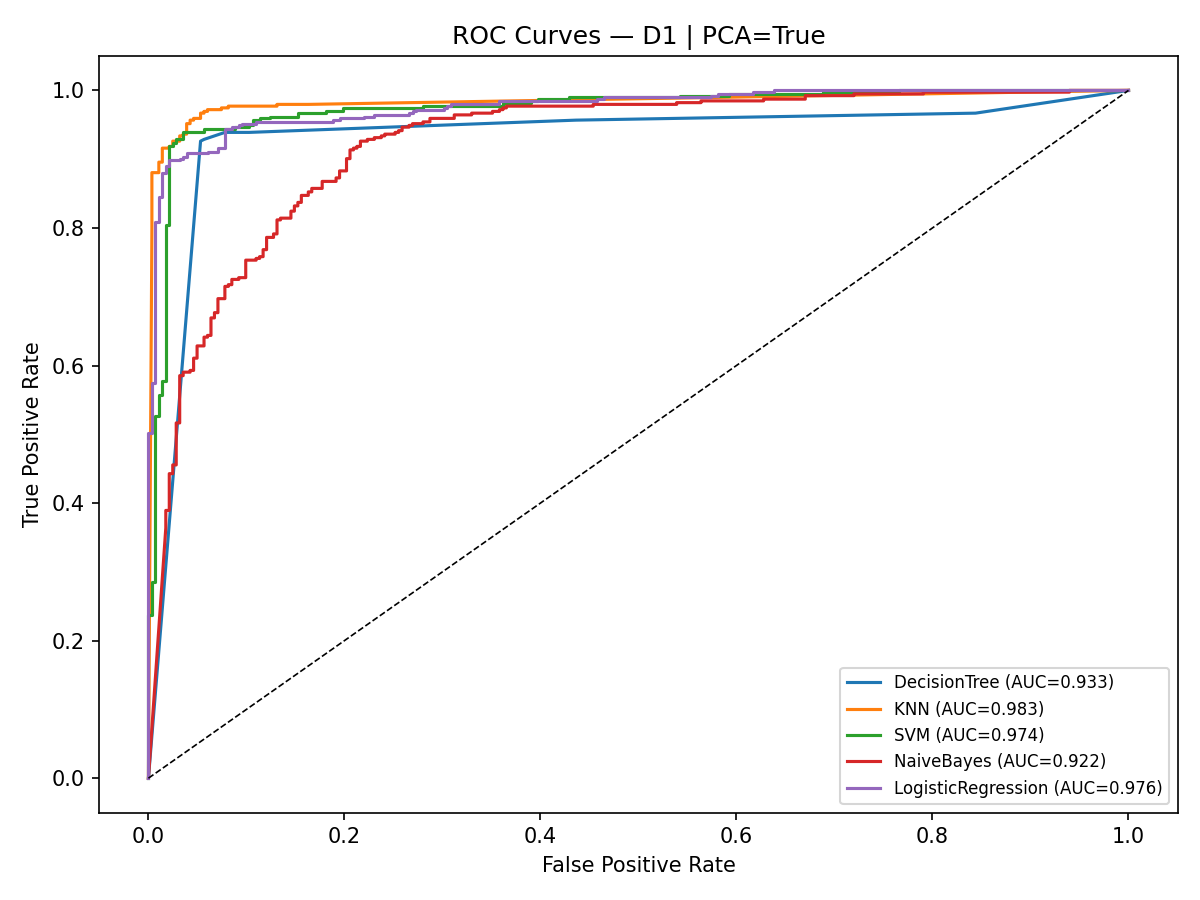
\includegraphics[width=\linewidth]{results/figures/D1_pca_roc.png}
    \caption{D1 — After PCA}
  \end{subfigure}
  \caption{ROC curves on the D1 dataset. SVM achieves the highest AUC on raw features (0.982). After PCA, curves converge and NB degrades substantially.}
  \label{fig:d1_roc}
\end{figure}

\subsection{Results on D2}

D2 is the VLD-deduplicated, perfectly balanced variant of D1. Its results are reported in Table~\ref{tab:d2}.

\begin{table}[H]
\centering
\caption{Phase I results on D2 (2,238 samples). Best per column in \textbf{bold}.}
\label{tab:d2}
\renewcommand{\arraystretch}{1.15}
\begin{tabular}{@{}llccccc@{}}
\toprule
 & Model & Acc & Pre & Rec & F1 & AUC \\
\midrule
\multirow{5}{*}{\rotatebox{90}{Raw}}
 & DT   & \textbf{.953} & .959 & .946 & \textbf{.953} & .938 \\
 & KNN  & .940 & .967 & .911 & .938 & .977 \\
 & SVM  & .946 & .951 & .942 & .946 & \textbf{.985} \\
 & NB   & .799 & .965 & .621 & .755 & .952 \\
 & LR   & .944 & .950 & \textbf{.938} & .944 & .984 \\
\midrule
\multirow{5}{*}{\rotatebox{90}{PCA}}
 & DT   & .895 & .904 & .884 & .894 & .880 \\
 & KNN  & .944 & .976 & .911 & .942 & .974 \\
 & SVM  & .951 & .963 & .938 & \textbf{.950} & \textbf{.979} \\
 & NB   & .737 & .973 & .487 & .649 & .948 \\
 & LR   & .935 & .949 & .920 & .934 & .974 \\
\bottomrule
\end{tabular}
\end{table}

On D2, SVM records the highest AUC in both configurations (0.985 raw, 0.979 PCA). The class balance appears to benefit SVM and LR, both of which depend on linear or kernelised margin optimisation that is sensitive to class imbalance. Decision Tree degrades notably under PCA (F1 drops from 0.953 to 0.894), confirming that tree-based models prefer the original feature space.

\begin{figure}[H]
  \centering
  \begin{subfigure}[b]{0.48\linewidth}
    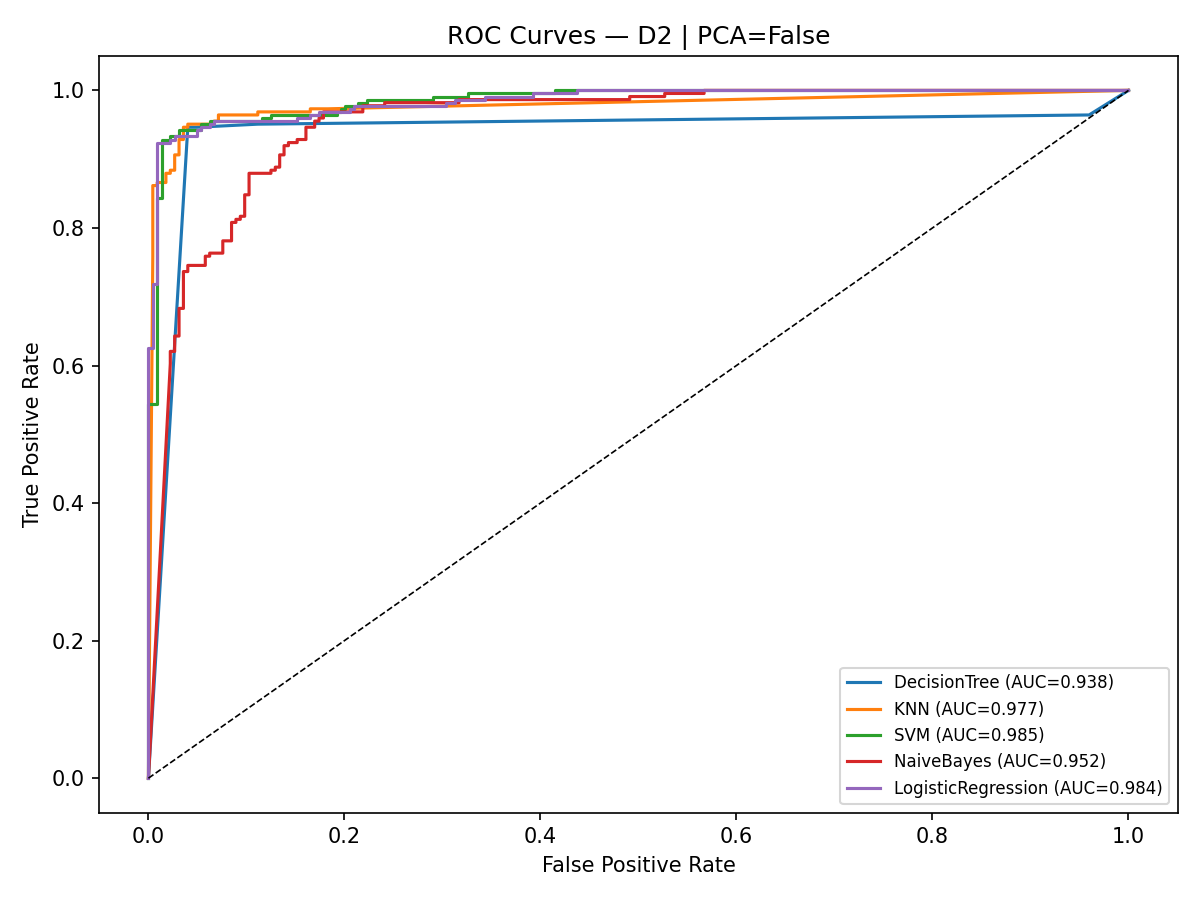
\includegraphics[width=\linewidth]{results/figures/D2_raw_roc.png}
    \caption{D2 — Raw features}
  \end{subfigure}
  \hfill
  \begin{subfigure}[b]{0.48\linewidth}
    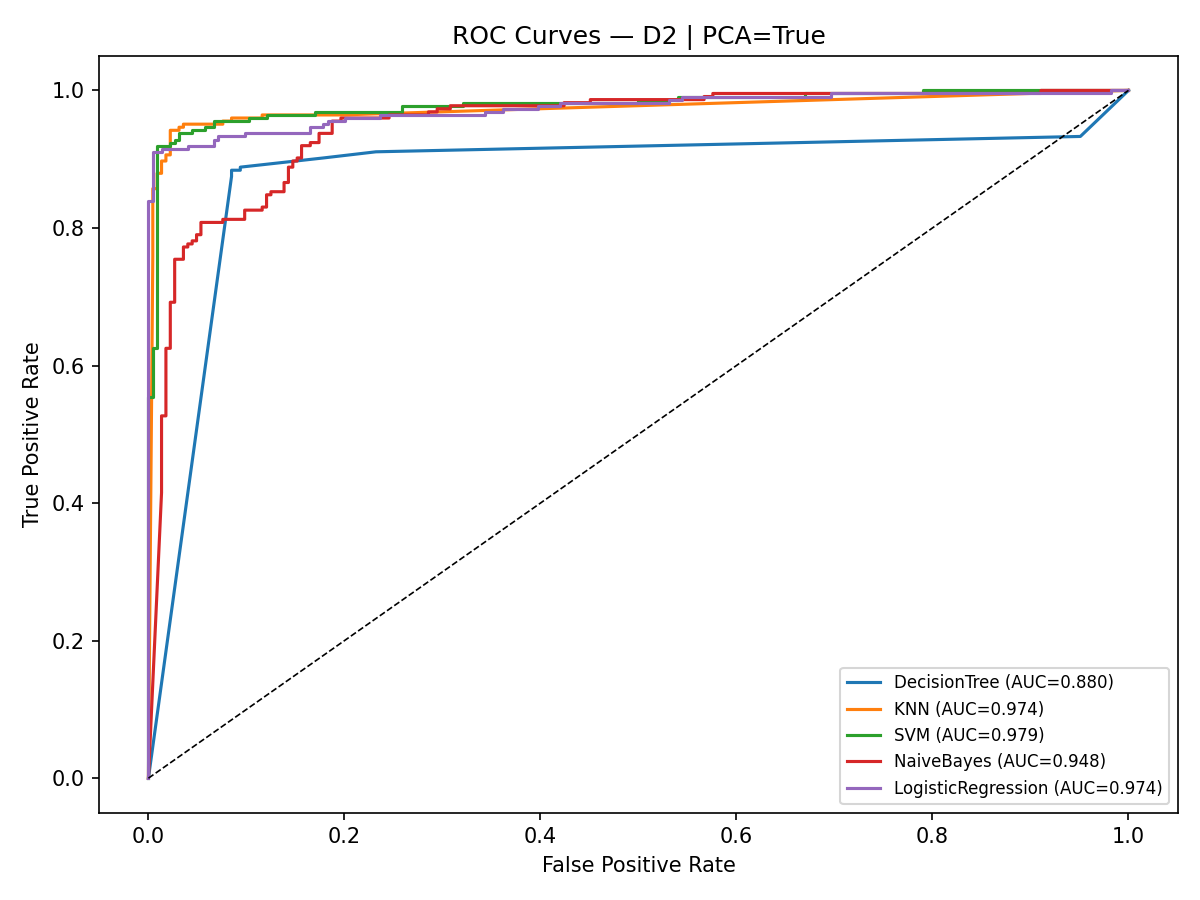
\includegraphics[width=\linewidth]{results/figures/D2_pca_roc.png}
    \caption{D2 — After PCA}
  \end{subfigure}
  \caption{ROC curves on the D2 dataset. SVM and LR dominate at high-AUC operating points. PCA maintains most of the discriminative signal for kernel methods.}
  \label{fig:d2_roc}
\end{figure}

\subsection{Correlation Structure of Pre-Extracted Features}

Fig.~\ref{fig:correlation} shows the Pearson correlation heatmap for the top 40 features of D2. Several dense clusters of highly correlated dangerous-function counts are visible (deep blue and deep red blocks). These clusters justify the use of PCA and feature selection to reduce redundancy, even if both interventions hurt tree-based models here.

\onecolumn
\begin{figure}[H]
  \centering
  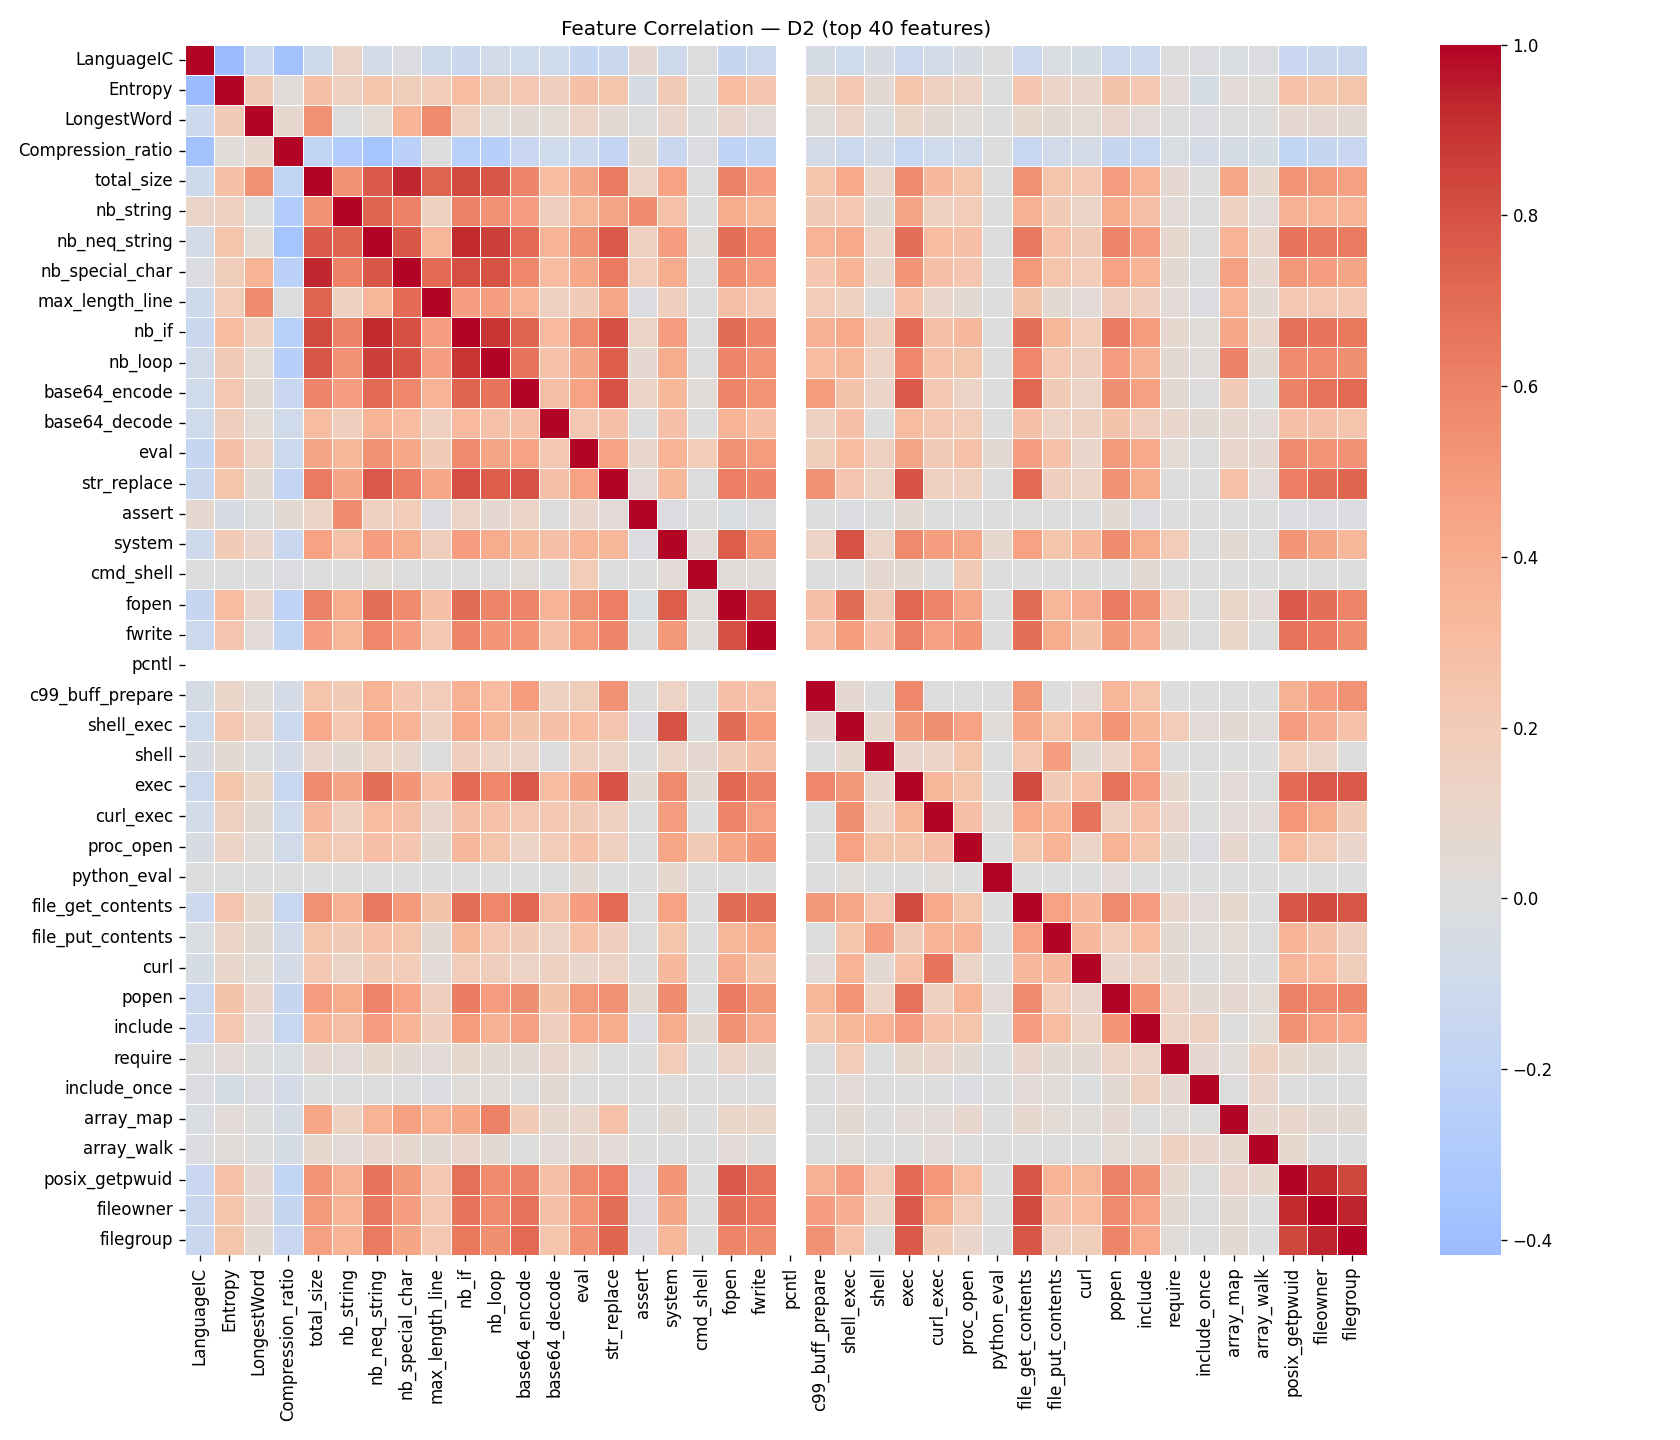
\includegraphics[width=0.78\textwidth]{results/figures/D2_correlation.png}
  \caption{Pearson correlation heatmap for the top 40 features of D2. Clusters of co-occurring dangerous functions (e.g.\ \texttt{eval}/\texttt{base64\_decode}/\texttt{assert}) produce high positive correlations. The \texttt{label} column is excluded.}
  \label{fig:correlation}
\end{figure}
\twocolumn

% ============================================================
\section{Phase II: WhiteBlackPHP with Custom Feature Extraction}
% ============================================================

\subsection{Feature Importance Analysis}

Before training classifiers, Random Forest is used as an embedded feature selector to rank the 87 extracted features by their mean decrease in impurity. Fig.~\ref{fig:rf_importance} presents the top 30 most discriminative features.

\onecolumn
\begin{figure}[H]
  \centering
  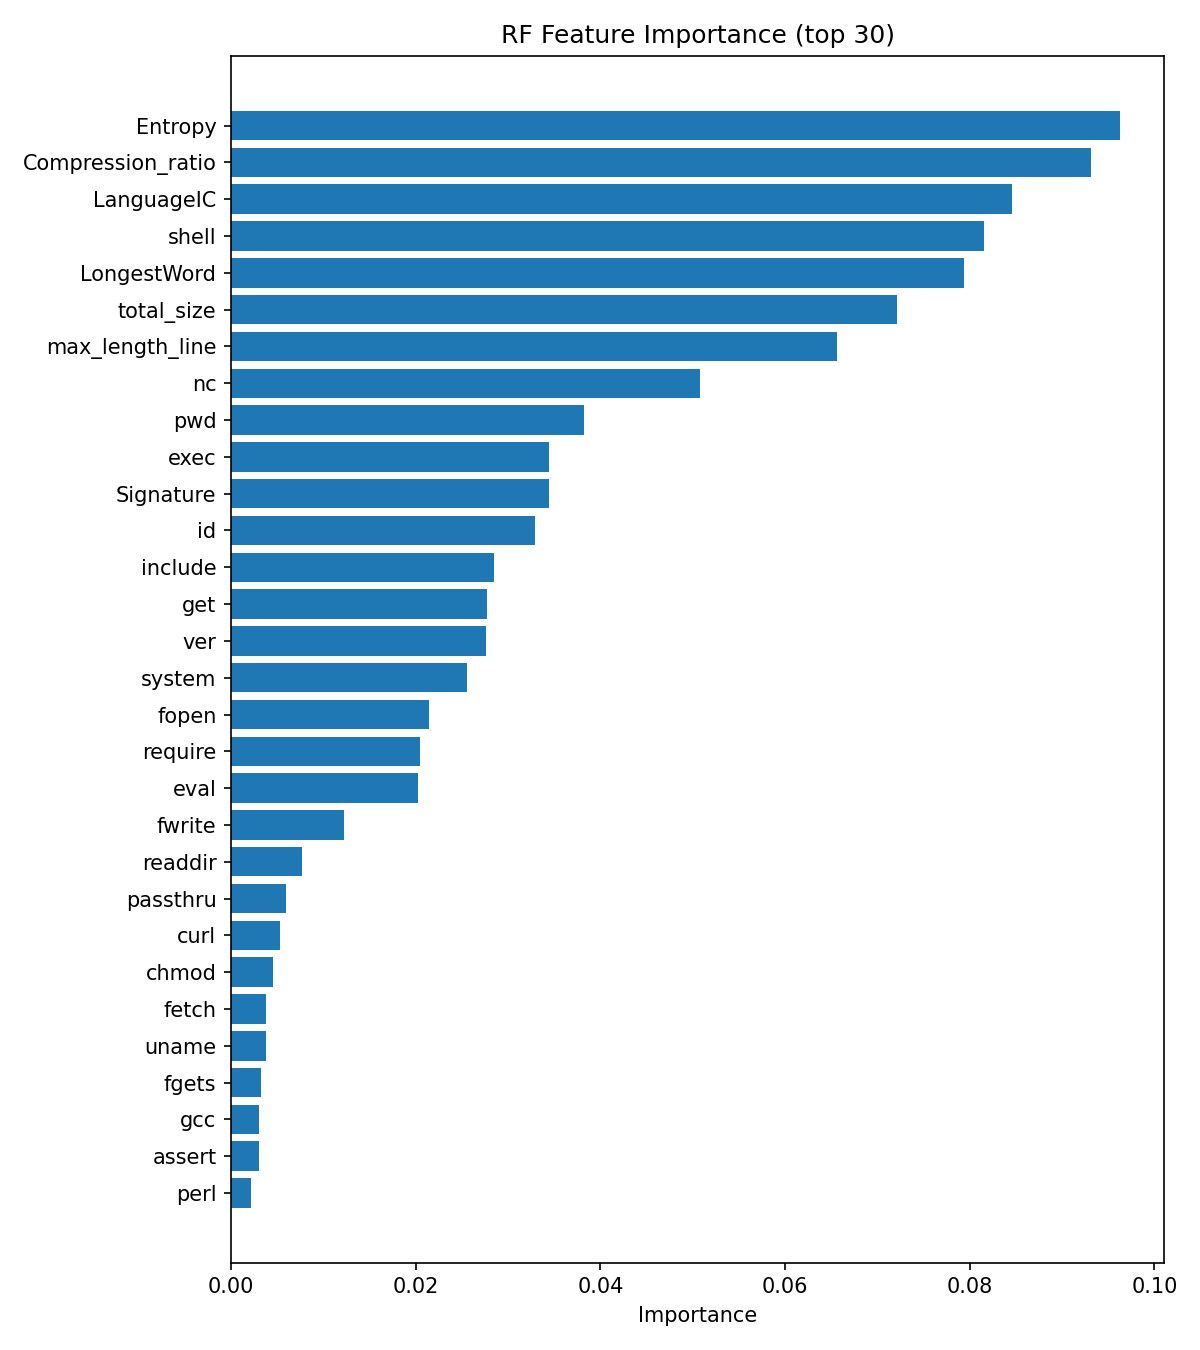
\includegraphics[width=0.78\textwidth]{results/figures/part2_rf_importance.png}
  \caption{Top-30 feature importances from a Random Forest trained on the full WhiteBlackPHP feature set. Statistical features (Entropy, Compression\_ratio, LanguageIC) and lexical features (\texttt{eval}, \texttt{base64\_decode}, \texttt{\$\_POST}) dominate. Purely syntactical features such as \texttt{nb\_if} contribute less.}
  \label{fig:rf_importance}
\end{figure}
\twocolumn

Statistical features (Entropy, Compression ratio, Index of Coincidence) appear among the top discriminators, validating the neopi hypothesis. Among lexical features, \texttt{eval}, \texttt{base64\_decode}, \texttt{assert}, and \texttt{\$\_POST} are consistently ranked high. Syntactical features such as \texttt{nb\_if} contribute less individually but improve model calibration collectively.

\subsection{Results Without Feature Selection}

Table~\ref{tab:part2_nofs} reports the seven-classifier comparison on the full 87-feature set extracted from the WhiteBlackPHP dataset.

\begin{table}[H]
\centering
\caption{Phase II results on WhiteBlackPHP --- Full feature set (87 features). Best per column in \textbf{bold}.}
\label{tab:part2_nofs}
\renewcommand{\arraystretch}{1.15}
\begin{tabular}{@{}lccccc@{}}
\toprule
Model & Acc & Pre & Rec & F1 & AUC \\
\midrule
DT              & .941 & .930 & .953 & .941 & .941 \\
KNN             & .942 & .952 & .932 & .942 & .982 \\
SVM             & .931 & .957 & .902 & .929 & .975 \\
NB              & .699 & .988 & .403 & .572 & .922 \\
LR              & .919 & .939 & .897 & .917 & .969 \\
RF              & \textbf{.966} & \textbf{.969} & \textbf{.963} & \textbf{.966} & \textbf{.995} \\
AdaCost         & .928 & .958 & .896 & .926 & .977 \\
\bottomrule
\end{tabular}
\end{table}

Random Forest is the undisputed winner, achieving F1 = 0.966 and AUC = 0.995. The near-perfect AUC means that at any operating threshold, the model successfully separates the two classes. AdaCost reaches AUC = 0.977 with precision of 0.958, making it a viable choice when the cost of false negatives must be explicitly controlled. NB again collapses in recall (0.403), confirming that the strong feature correlation structure violates its independence assumption.

Fig.~\ref{fig:part2_nofs_roc} shows the ROC curves for all seven classifiers.

\begin{figure}[H]
  \centering
  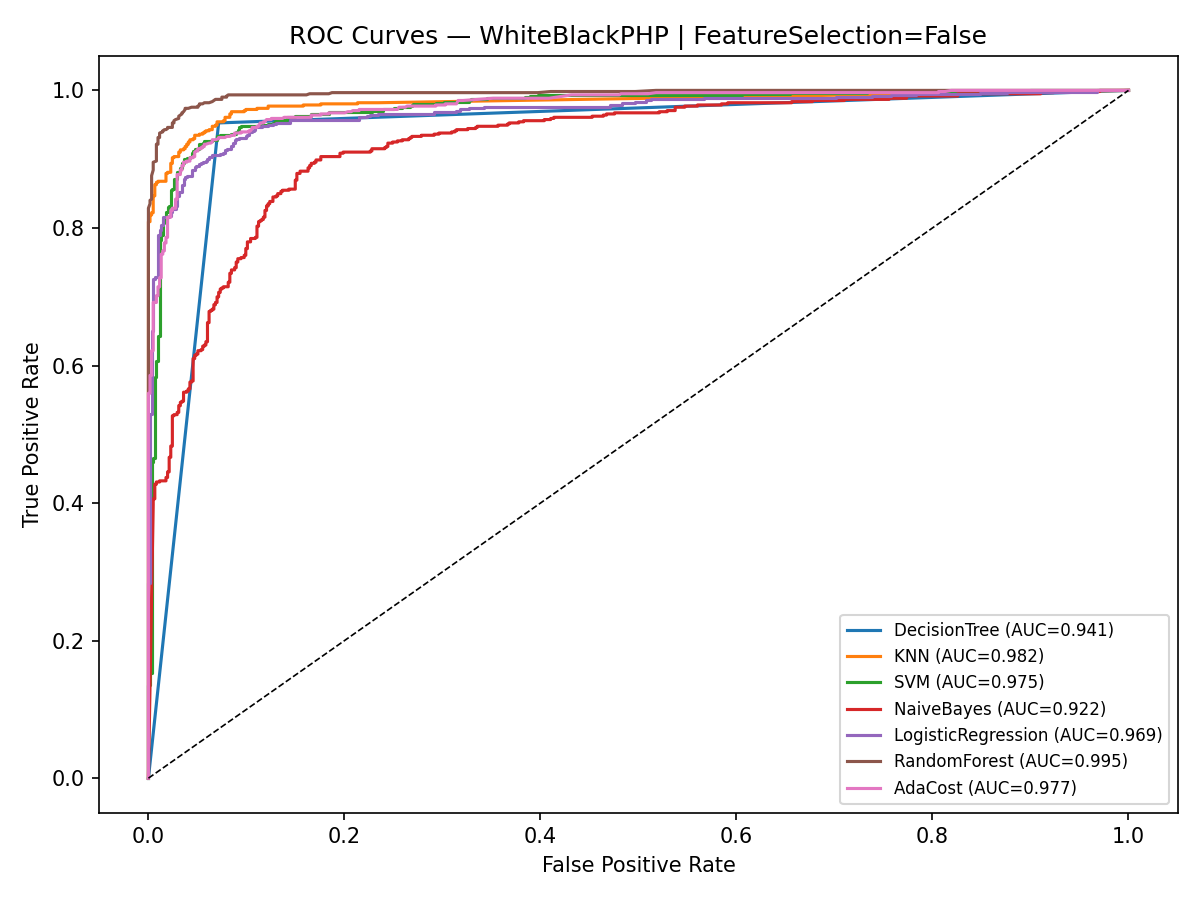
\includegraphics[width=\linewidth]{results/figures/part2_no_fs_roc.png}
  \caption{ROC curves on WhiteBlackPHP without feature selection. Random Forest (AUC 0.995) and KNN (AUC 0.982) dominate the curve. NB achieves high precision at very low recall.}
  \label{fig:part2_nofs_roc}
\end{figure}

\subsection{Results With Feature Selection}

Table~\ref{tab:part2_fs} reports the same seven classifiers after reducing the feature space to the top 30 features by F-score.

\begin{table}[H]
\centering
\caption{Phase II results on WhiteBlackPHP --- SelectKBest top-30 features. Best per column in \textbf{bold}.}
\label{tab:part2_fs}
\renewcommand{\arraystretch}{1.15}
\begin{tabular}{@{}lccccc@{}}
\toprule
Model & Acc & Pre & Rec & F1 & AUC \\
\midrule
DT              & .900 & .898 & .902 & .900 & .915 \\
KNN             & .915 & .924 & .905 & .914 & .957 \\
SVM             & .884 & .952 & .808 & .874 & .951 \\
NB              & .681 & .963 & .377 & .542 & .916 \\
LR              & .863 & .905 & .811 & .855 & .934 \\
RF              & \textbf{.948} & \textbf{.955} & \textbf{.940} & \textbf{.947} & \textbf{.988} \\
AdaCost         & .893 & .940 & .840 & .887 & .957 \\
\bottomrule
\end{tabular}
\end{table}

Feature selection uniformly reduces performance across all models. Random Forest drops from F1 = 0.966 to 0.947; AdaCost drops from 0.926 to 0.887. This result is instructive: the 87-feature set is already compact, and the features eliminated by SelectKBest (the lower-ranked lexical keyword counts) still carry marginal but non-negligible discriminative information. Ensemble methods, which implicitly perform internal feature selection, suffer less from this reduction.

Fig.~\ref{fig:part2_comparison} juxtaposes the metric profiles of all seven classifiers under both configurations.

\onecolumn
\begin{figure}[H]
  \centering
  \begin{subfigure}[b]{0.48\textwidth}
    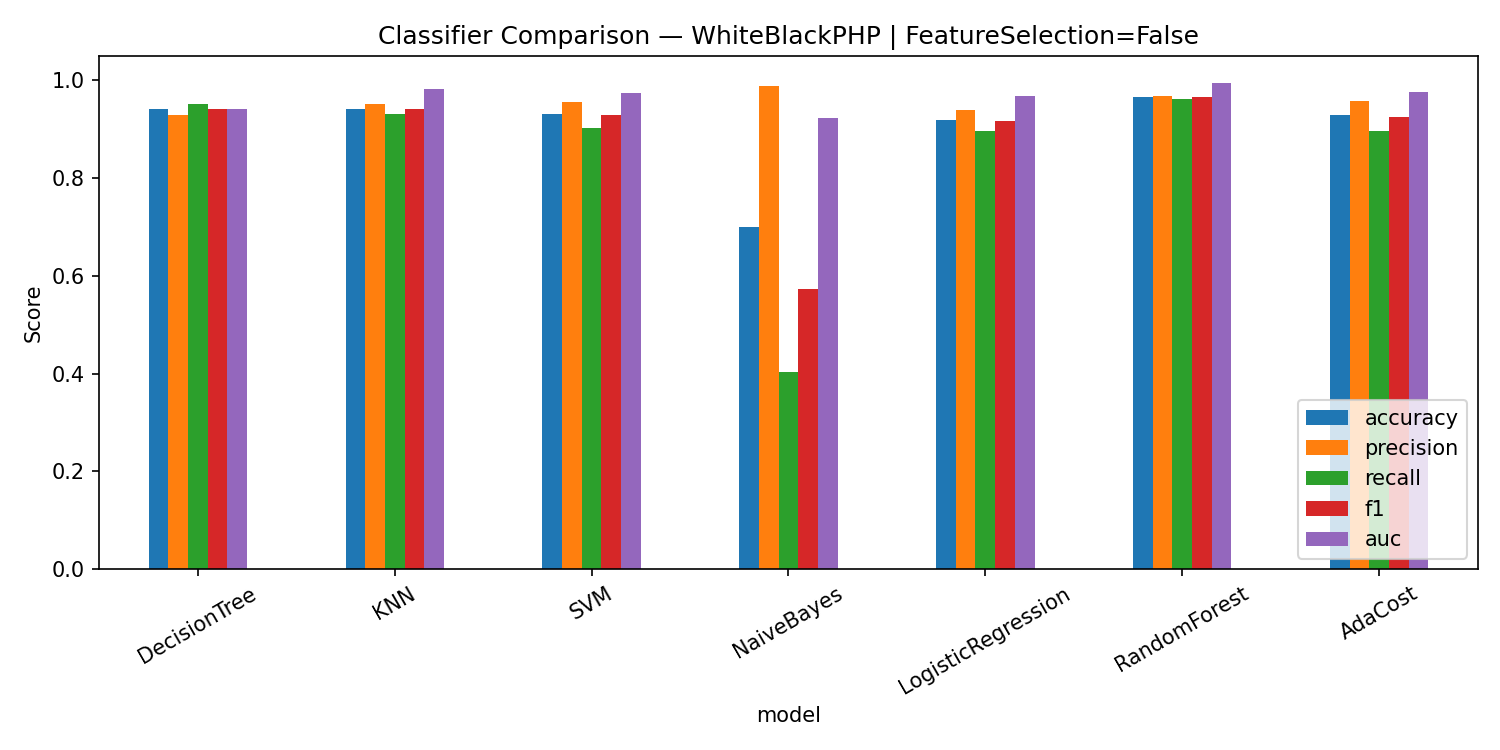
\includegraphics[width=\linewidth]{results/figures/part2_no_fs_comparison.png}
    \caption{Full feature set (87 features)}
  \end{subfigure}
  \hfill
  \begin{subfigure}[b]{0.48\textwidth}
    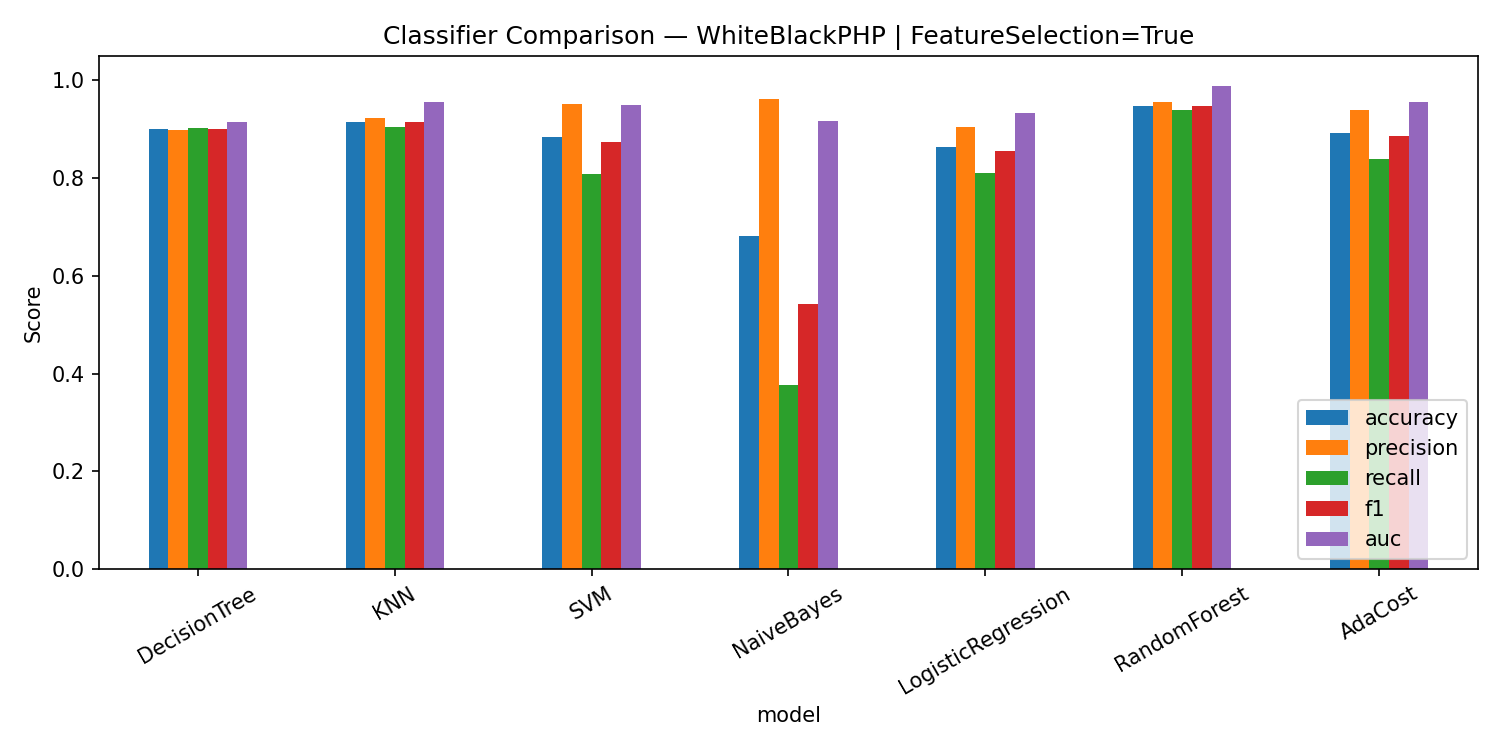
\includegraphics[width=\linewidth]{results/figures/part2_with_fs_comparison.png}
    \caption{SelectKBest top-30 features}
  \end{subfigure}
  \caption{Multi-metric comparison of all seven classifiers on WhiteBlackPHP. Feature selection consistently lowers every metric for every model. Random Forest is the most robust. NB achieves high precision at the cost of extremely low recall in both settings.}
  \label{fig:part2_comparison}
\end{figure}
\twocolumn

% ============================================================
\section{Discussion}
% ============================================================

\subsection{Effect of PCA and Feature Selection}

PCA and SelectKBest both reduce the effective dimensionality of the feature space. In our experiments, both consistently reduce recall---the most security-critical metric---without substantially improving precision. The root cause is information loss: both transformations discard features that, while noisy or correlated with others, still carry partial signal about rare obfuscated webshells.

The exception is KNN on D1 under PCA, where AUC increases from 0.975 to 0.983. Euclidean distances in high-dimensional, correlated feature spaces are dominated by irrelevant directions, so removing them via PCA genuinely improves neighbourhood quality. For tree-based and linear models, the original standardised feature space is preferable.

\subsection{Na\"{i}ve Bayes and Feature Correlation}

NB consistently achieves the highest precision in our experiments---often above 0.96---but the lowest recall. The correlation heatmap (Fig.~\ref{fig:correlation}) explains why: features such as \texttt{eval} and \texttt{base64\_decode} almost always co-occur, violently violating the Gaussian independence assumption. NB's likelihood function double-counts this evidence, making it extremely conservative and reluctant to flag a file as a webshell unless the evidence is overwhelming. This pathology worsens on the WhiteBlackPHP dataset, where the feature set is even more correlated.

\subsection{Ensemble Methods and Cost-Sensitivity}

Random Forest's superiority is attributable to two mechanisms: variance reduction through bagging, and implicit feature selection through random subspace sampling. With 87 features and thousands of trees, each tree focuses on a different subset of the feature space, collectively building a robust boundary that generalises well.

AdaCost was designed to minimise the false-negative rate by assigning higher misclassification cost to webshells. In our experiments, AdaCost with $c^+ = 3$ or $c^+ = 5$ achieves higher recall than SVM or LR but slightly lower than RF. In production security systems, where a missed webshell is far more dangerous than a false alert, AdaCost provides a principled mechanism to tune the precision-recall trade-off without threshold post-processing.

\subsection{Cross-Dataset Consistency}

Comparing Phase I (pre-extracted features) and Phase II (custom extraction), the relative ordering of classifiers is largely preserved: RF $>$ DT $\approx$ KNN $>$ SVM $>$ LR $>$ AdaCost $\gg$ NB. This consistency validates both the feature extraction pipeline and the model implementations. The custom-extracted features in Phase II are competitive with the pre-extracted D1/D2 features despite being derived from raw text, confirming that the feature engineering design is sound.

% ============================================================
\section{Conclusion}
% ============================================================

This paper presented a comprehensive machine learning study for PHP webshell detection, covering three independent datasets, two preprocessing configurations, custom feature engineering, and seven classifiers. The main findings are:

\begin{enumerate}
  \item \textbf{Random Forest achieves the best results} across all experiments (F1 = 0.966, AUC = 0.995 on WhiteBlackPHP), establishing it as the recommended baseline for PHP webshell detection.
  \item \textbf{Feature selection and PCA degrade performance}: the 87-feature set is already compact enough that dimensionality reduction loses more signal than it removes noise.
  \item \textbf{Na\"{i}ve Bayes is unsuitable} for this feature space due to severe inter-feature correlation, manifesting as catastrophic recall collapse ($<$ 0.41).
  \item \textbf{Statistical features are the most discriminative}: entropy, compression ratio, and IC consistently rank at the top of the RF importance ranking, validating the neopi approach.
  \item \textbf{AdaCost provides principled cost sensitivity}: its ability to penalise false negatives makes it valuable when the operational cost of missing a webshell exceeds the cost of a false alert.
\end{enumerate}

Future work will extend this study to deep learning models operating on raw byte sequences, investigate adversarial robustness under the four evasion techniques described in Section~I, and integrate the classifier into a live web application firewall pipeline for real-time detection.

% ============================================================
\appendix
% ============================================================

\section{AdaCost Algorithm}

Algorithm~\ref{alg:adacost} provides the pseudocode for AdaCost as implemented in this work.

\begin{algorithm}[H]
\caption{AdaCost (Fan et al., 1999)}
\label{alg:adacost}
\begin{algorithmic}[1]
\REQUIRE Training set $\{(x_i, y_i)\}_{i=1}^n$, $y_i \in \{-1, +1\}$\\
\REQUIRE Cost parameters $c^+$ (FN cost), $c^-$ (FP cost)\\
\REQUIRE Number of rounds $T$
\STATE Initialise $w_i = 1/n$ for all $i$
\FOR{$t = 1$ to $T$}
  \STATE Fit weak learner $h_t$ using weights $w_i$
  \STATE $\varepsilon_t = \sum_i w_i \cdot \mathbb{1}[h_t(x_i) \neq y_i]$
  \IF{$\varepsilon_t \geq 0.5$ or $\varepsilon_t = 0$}
    \STATE \textbf{break}
  \ENDIF
  \STATE $\alpha_t = \frac{1}{2}\ln\frac{1 - \varepsilon_t}{\varepsilon_t}$
  \FOR{each sample $i$}
    \STATE $\beta_i \leftarrow c^+$ if FN, $c^-$ if FP, else $1$
    \STATE $w_i \leftarrow w_i \exp(\alpha_t \cdot \mathbb{1}[\text{wrong}] \cdot \beta_i)$
  \ENDFOR
  \STATE Normalise $w_i \leftarrow w_i / \sum_j w_j$
\ENDFOR
\RETURN $H(x) = \text{sign}\!\left(\sum_t \alpha_t h_t(x)\right)$
\end{algorithmic}
\end{algorithm}

% ============================================================
\begin{thebibliography}{99}

\bibitem{wang2012detecting}
Y.~Wang, W.~Tang, Y.~Li, and Z.~Mao,
``Detecting webshell via statistical features of HTTP requests and shell scripts,''
in \textit{Proc.\ International Workshop on Cyber Security},
2012.

\bibitem{wang2015detecting}
Z.~Wang, Y.~Chen, D.~Wang, and X.~Zhong,
``Detecting webshell attacks through machine learning methods,''
in \textit{Proc.\ IEEE Trustcom/BigDataSE/ISPA}, vol.~1, pp.~150--159, 2015.

\bibitem{fan1999adacost}
W.~Fan, S.~J.~Stolfo, J.~Zhang, and P.~K.~Chan,
``AdaCost: Misclassification cost-sensitive boosting,''
in \textit{Proc.\ ICML}, vol.~99, pp.~97--105, 1999.

\bibitem{neopi2010}
B.~Carn\`{e} and R.~Sisto,
``neopi: Detecting potentially malicious PHP files,''
\textit{Google Code Archive},
2010.
[Online]. Available: \url{https://code.google.com/archive/p/neo-pi/}

\bibitem{tian2020}
Z.~Tian, C.~Luo, J.~Qiu, X.~Du, and M.~Guizani,
``A distributed deep learning system for web attack detection on edge devices,''
\textit{IEEE Trans.\ Industrial Informatics}, vol.~16, no.~3, pp.~1963--1971, 2020.

\bibitem{dataset2022}
M.~Riadh and R.~Djahida,
``WhiteBlackPHP: A benchmark dataset for PHP webshell detection,''
\textit{Mendeley Data}, v2,
2022.
[Online]. Available: \url{https://data.mendeley.com/datasets/wt8m6bcwbr/2}

\bibitem{breiman2001rf}
L.~Breiman,
``Random forests,''
\textit{Machine Learning}, vol.~45, no.~1, pp.~5--32, 2001.

\bibitem{cortes1995svm}
C.~Cortes and V.~Vapnik,
``Support-vector networks,''
\textit{Machine Learning}, vol.~20, no.~3, pp.~273--297, 1995.

\end{thebibliography}

\end{document}
